\subsection{Traitement d'un intrant vocal}
La première étape de calcul au sein d’une architecture neurale destinée à comprendre et répondre à un utilisateur est de comprendre ce qu’il dit. Pour accomplir cette tâche, il est possible d’utiliser un réseaux de neurones TC-DNN-BLSTM-DNN, c’est-à-dire, des convolutions temporelles (TC) suivies de couches de neurones linéaires profondes (DNN), d’un LSTM Bidirectionnel (BLSTM) et puis d’un second DNN final \cite{acousticModeling}. Ainsi, cette architecture dépend d’un pré-traitement du signal par un autre algorithme lequel est plus classique et permet de transformer le signal en un domaine de fréquences personnalisées. C’est ce pré-traitement de l’information qui est introduit dans le réseau de neurones profond, afin d’en analyser le sens et de pouvoir convertir cela en états acoustiques, lesquels peuvent être convertis, cette fois, en texte littéraire. Cette architecture neurale, imagée à la \autoref{fig:tcDnnBlstmDnn}, obtient un WER (Word Error Rate) de retranscription de 3.47, ce qui est présentement l’état de l’art (SOTA) sur le jeux de données et problème du Wall Street Journal (WSJ) eval’92 \\%[PAPER REQUIS POUR LE WSJ eval’92, CITATION].

\begin{figure*}
  \centering
  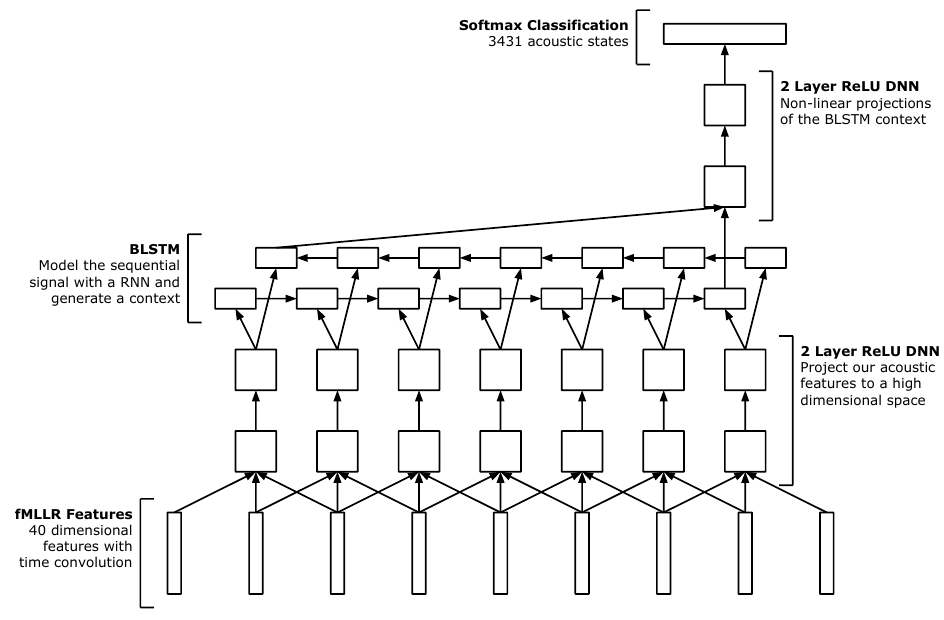
\includegraphics[width=\textwidth]{tcDnnBlstmDnn}
  \caption{Architecture neurale TC-DNN-BLSTM-DNN [rajouter reference ici]}
  \label{fig:tcDnnBlstmDnn}
\end{figure*}

L’architecture neurale TC-DNN-BLSTM-DNN permet d’écouter le signal audio à l’aide des données audio extraites en fMMLR. Ainsi, un DNN suivi d’un BLSTM peut analyser ce signal pour classifier cela en états acoustiques, lesquels sont eux-mêmes repris par un algorithme classique qui permet de rassembler ces états en mots réels [DeepRecurrentNeuralNetworksForAcousticModelling]. Notons que cette architecture neural peut être utilisée pour raffiner le signal des mots prononcés, ce qui peut être envoyé directement dans un réseaux de neurones supérieur en tant que plongeage.
